\chapter{Zwei-Faktor-Authentifizierungsmethoden}

Die \ac{2FA} ist ein Sicherheitsverfahren, welches zwei unterschiedliche Komponenten zur Verifizierung der Identität von Nutzerinnen erfordert \parencite{decristofaroComparativeUsability2014}. Verschiedene Publikationen definieren dazu drei Kategorien \parencite{decristofaroComparativeUsability2014, yuEfficientGeneric2014, singhMultifactorAuthentication2017}:
\begin{itemize}
  \item \textbf{Wissen}: Etwas, was die Benutzerin weiß (z.B. Passwort, PIN)
  \item \textbf{Besitz}: Etwas, was die Benutzerin besitzt (z.B. Smartphone, Physisches Token)
  \item \textbf{Inhärenz}: Etwas, was die Benutzerin ist (z.B. Fingerabdruck, Gesichtserkennung)
\end{itemize}
Sobald Elemente aus verschiedenen Kategorien genutzt werden, handelt es sich um Multi-Faktor-Authentifizierung. Am meisten verbreitet ist \ac{2FA}, wobei Faktoren aus zwei der Kategorien abgefragt werden \parencite{decristofaroComparativeUsability2014}. Am Häufigsten wird \ac{2FA} mit einen Passwort und einem weiteren Faktor umgesetzt \parencite{decristofaroComparativeUsability2014}.

\pskip
\ac{2FA} stellt eine Verbesserung der Sicherheit gegenüber traditionellen Methoden, die nur einen Faktor verwenden (z.B. Passwörter), da es schwieriger ist, beide Faktoren zu kompromittieren \parencite{dasguptaMultiFactorAuthentication2017}.

Des Weiteren werden gängige Angriffsmethoden wie Phishing oder Keylogging erschwert. Angreiferinnen können selbst wenn sie das Passwort wissen, nicht auf die Konten der Benutzerinnen zugreifen \parencite{dasguptaMultiFactorAuthentication2017}. Auch wenn Passwörter im Rahmen eines Daten-Leaks an die Öffentlichkeit geraten, ermöglicht dies keinen sofortigen Zugriff und gibt den Betroffenen Zeit, ihr Passwort anzupassen.

\pskip
In vielen Bereichen, wie beispielsweise dem Online-Banking und Regierungsbehörden, wird \ac{2FA} eingesetzt und ist Pflicht. \textcite{decristofaroComparativeUsability2014} identifizieren drei Bereiche, in denen \ac{2FA} hauptsächlich genutzt wird: im Privaten, in Finanzanwendungen und auf der Arbeit. Dennoch ist die Entwicklung von \ac{2FA}-Methoden noch nicht abgeschlossen und birgt einige Herausforderungen.

Einerseits kann die Einführung eines zusätzlichen Authentifizierungsschrittes zu Lasten der Benutzerinnenerfahrung gehen \parencite{decristofaroComparativeUsability2014}. Andererseits werden durch zusätzliche Faktoren auch zusätzliche Implementierungskosten hervorgerufen, sei dies durch Hardware-Kosten (z.B. für Security Keys), technische Implementierung, oder Support \parencite{alsaleemMultiFactorAuthentication2021}.

\pskip
Im folgenden werden fünf gängige \ac{2FA}-Methoden vorgestellt. Dabei wird sowohl auf deren Funktionsweise, als auch auf Usability-Probleme und Sicherheitserwägungen eingegangen.

\section{OTPs über SMS/Email}
\label{sec:otp}

Die laut einer Studie von \citeyear{decristofaroComparativeUsability2014} am häufigsten verbreitete \ac{2FA}-Methode sind \acp{OTP} über SMS und Email \parencite{decristofaroComparativeUsability2014}\footnote{Nur im professionellen Kontext werden Hardware-Tokens mehr als \acp{OTP} über SMS und Email verwendet \parencite{decristofaroComparativeUsability2014}.}. Dabei handelt es sich um immer wieder neu generierte Passwörter oder PINs, die zusätzlich zu einem statischen Passwort angegeben werden müssen \parencite{geramiOneTimePasswords2016}. Das \ac{OTP} wird während des Login-Versuches auf dem Server generiert und über \acs{SMS} oder Email an die Nutzerin gesendet. Es ist nur einmalig nutzbar und verfällt in den meisten Fällen nach einer bestimmten Zeit \parencite{geramiOneTimePasswords2016}. Nach erfolgter Eingabe gleicht der Server das eingegebene \ac{OTP} mit dem zuvor generierten ab und beendet den Login-Vorgang mit Zulassung oder Abweisung.

Die Nutzung von \acp{OTP}, die über SMS oder Email zugestellt werden ist weit verbreitet \parencite{decristofaroComparativeUsability2014}. Grund dafür ist die einfache Nutzung, die keine zusätzlichen Geräte oder zusätzliche Software benötigt \parencite{abhishekComprehensiveStudy2013}. Des Weiteren ist es einfach, diese Authentifzierungsmethode einzurichten, da es nur nötig ist, die Telefonnummer oder Email-Adresse der Nutzerin abzufragen. Auch die Implementierungskosten halten sich in Grenzen \parencite{abhishekComprehensiveStudy2013}.

\subsubsection{Sicherheitsaspekte}

\ac{OTP} ist im Allgemeinen resistent gegen Attacken wie Key-Logger und "Shoulder Surfing", da die Einmalpasswörter nach der ersten Benutzung verfallen \parencite{abhishekComprehensiveStudy2013}. Aus dem gleichen Grund können auch traditionelle Phishing-Attacken, welche Zugangsdaten abspeichern, um sie zu einem späteren Zeitpunkt wieder zu nutzen, gestoppt werden. Während Echtzeit-Phishing schwieriger umzusetzen ist, ist es auch schwieriger zu stoppen \parencite{langSecurityKeys2017}.

Des Weiteren sind \acp{OTP} aufgrund des begrenzten Zeitfensters der Nutzung relativ unanfällig gegenüber Brute-Force-Attacken \parencite{reeseUsabilityStudy2019}. Auf dem Server müssen die Einmalpasswörter sicher gespeichert werden, dabei kann aber ein Hashing-Algorithmus hilfreich sein \parencite{reeseUsabilityStudy2019}.

\ac{MIM}-Attacken können jedoch durch \ac{OTP} nicht verhindert werden. Eine dritte Partei kann sich weiterhin als die Anwendung ausgeben, bei der sich die Nutzerin anmelden will und dann ihre Angaben annehmen und an die echte Anwendung weitergeben. Somit ist es auch möglich, sich Zugriff zum Konto der Nutzerin zu verschaffen, indem auch das \ac{OTP} entgegengenommen und im Namen der Nutzerin übermittelt wird.

\pskip
Außerdem muss sichergestellt werden, dass der gewählte Übertragungskanal für das \ac{OTP} sicher ist \parencite{abhishekComprehensiveStudy2013}. Eine Kompromittierung des statischen Passworts und des Übertragungskanals kann dazu führen, dass Angreiferinnen sich Zugriff verschaffen, indem sie einen Login-Versuch starten, das \ac{OTP} abfangen und dieses nutzen.

Das häufig genutzte SMS-Protokoll stellt einen unsicheren Übertragungskanal dar \parencite{peetersSMSOTP2022}. Einerseits ist die Übertragung von SMS-Nachrichten größtenteils unverschlüsselt, mit der möglichen Ausnahme der Wegstrecke zwischen Sendemast und Mobiltelefon \parencite{peetersSMSOTP2022}. Andererseits existieren verschiedene \textit{redirection attacks}, bei denen böswillige Parteien Zugriff auf fremde Nachrichten erhalten können \parencite{peetersSMSOTP2022}. Dazu gehört \textit{Sim Swapping}, wobei durch Social Engineering die Kontrolle über eine Telefonnummer auf eine SIM-Karte im Besitz der Angreiferinnen übertragen wird \parencite{leeEmpiricalStudy2020}. In einer Studie von \textcite{leeEmpiricalStudy2020} wurde festgestellt, dass alle untersuchten Mobilfunkbetreiber unsichere Authentifizierungsmethoden verwenden. Dies wird darauf zurückgeführt, dass die Konzerne eine bessere Usability über die Sicherheit der Nutzerinnen stellen. Eine weitere Gruppe von \textit{redirection attacks} nutzen Schwächen im \ac{SS7}-Protokoll aus, um ohne das Wissen der Nutzerinnen auf deren Nachrichten, Standorte und Anrufe zuzugreifen \parencite{ullahSS7Vulnerabilities2020}.

Auch die Übertragung von \acp{OTP} über Email stellt ein Sicherheitsrisiko dar. Einerseits verfügen viele Email-Konten nicht über \ac{2FA}, sind mit schwachen Passwörtern gesichert und besitzen Schwachstellen im Wiederherstellungsprozess \parencite{khannaAnatomyCompromising2012}. Andererseits sind Phishing-Attacken weiterhin ein beliebtes Mittel, bei dem menschliche Emotionen wie Verlustangst oder Gewinnerwartung genutzt werden, um Nutzerinnen zur Eingabe von Zugangsdaten zu bringen \parencite{goelGotPhished2017}.

\pskip
Während die Verwendung von \acp{OTP} über SMS und Email eine bessere Absicherung von Nutzerinnenkonten als ohne \ac{2FA} darstellt, existieren Methoden, die weitaus resistenter gegenüber bösartigen Attacken sind. In Abschnitt \ref{sec:totp} wird mit \ac{TOTP} auf eine solche Alternative eingegangen. Dabei fällt die Übermittlung der Einmalpasswörter vom Server an die Nutzerinnen weg, wodurch einige Angriffsvektoren ausgeschlossen werden können.

\subsubsection{Usability}

Da Textnachrichten einen zentralen Bestandteil im Leben vieler Nutzerinnen spielen, bevorzugen sie die Verwendung von \acp{OTP} über SMS gegenüber Alternativen \parencite{peetersSMSOTP2022}. Gleiches kann auch über Emails behauptet werden, da diese wohlbekannt und komfortabel zu nutzen sind \parencite{vishwakarmaSecureImage2016}. Meistens sind SMS-Nachrichten jedoch einfacher und schneller abzurufen, weshalb sie weiterhin bevorzugt werden \parencite{peetersSMSOTP2022}.

Eine Studie von \textcite{decristofaroComparativeUsability2014} stellte fest, dass Nutzerinnen einen Vorteil darin sahen, bereits vorhande Technologie für \ac{2FA} nutzen zu können. In Einzelfällen wurde SMS aus dem Grund bevorzugt, dass die Teilnehmerin nicht über ein Smartphone verfügte. Usability-Probleme bei der Nutzung von SMS traten im Zuge der Zustellung auf, bei der Verzögerungen und zusätzliche Kosten entstehen können \parencite{decristofaroComparativeUsability2014}.

Zu guter Letzt müssen die generierten Codes manuell eingegeben werden, was die Möglichkeit von Eingabefehlern mit sich bringt \parencite{decristofaroComparativeUsability2014}.

\section{TOTP}
\label{sec:totp}

\acfp{TOTP} verhalten sich in der Nutzungsweise ähnlich zu den in \ref{sec:otp} beschriebenen Einmalpasswörter. Bei \ac{TOTP} werden Einmalpasswörter ausgestellt, die eine beschränkte Lebenszeit haben \parencite{decristofaroComparativeUsability2014}. Meistens handelt es sich dabei um 6- oder 8-stellige Zahlenkombinationen, die von einer App auf dem Smartphone der Nutzerinnen generiert wird \parencite{decristofaroComparativeUsability2014}. Um \ac{TOTP} einzurichten, muss zuerst eine geeignete App (Aegis, Google Authenticator, etc.) installiert werden. In dieser App wird dann ein geheimer Schlüssel der Anwendung hinterlegt, was normalerweise über einen QR-Code geschieht \parencite{reeseUsabilityStudy2019}. Basierend auf dem geheimen Schlüssel und der aktuellen Uhrzeit generiert die App Codes, welche für je 30 Sekunden gültig sind und auf dem Server abgeglichen werden können \parencite{reeseUsabilityStudy2019}.

\subsubsection{Sicherheitsaspekte}

Der zur Verwendung von \ac{TOTP} benötigte geheime Schlüssel muss sowohl auf dem Server als auch auf dem Smartphone der Nutzerinnen sicher gespeichert werden \parencite{reeseUsabilityStudy2019}. Falls er kompromittiert wird und der genutzte Algorithmus bekannt ist, ist es Angreiferinnen möglich die Codes selbst zu generieren. Die Verwendung von Ein-Weg-Hashing zum Speichern des geheimen Schlüssel ist nicht möglich, da er zum Generieren und Verifizieren des Codes benötigt wird \parencite{reeseUsabilityStudy2019}. Auf dem Server könnte der Schlüssel allerdings mit dem Passwort der Nutzerinnen verschlüsselt werden \parencite{reeseUsabilityStudy2019}.

Die Anwendung, welche die \acp{TOTP} generiert, benötigt keinen Internetzugriff, und der Code wird nicht über eventuell unsichere Kanäle an die Nutzerin übermittelt \parencite{reeseUsabilityStudy2019}. Dies stellt einen Vorteil gegenüber herkömmlichen \acp{OTP} dar. Eine \ac{MIM}-Attacke ist allerdings weiterhin möglich, indem die Angreiferinnen die Anwendung nachstellen, Login-Daten abfangen und sofort selbst verwenden.

\subsubsection{Usability}

Im Vergleich zu \ac{OTP} werden mögliche Fehlerquellen reduziert, da keine Netzwerkverbindung benötigt wird \parencite{reeseUsabilityStudy2019}.

Da die Einmalpasswörter mit zeitlicher Beschränkung eingegeben werden müssen, gaben einige Teilnehmerinnen der Studie von \textcite{reeseUsabilityStudy2019} an, die Codes manchmal nicht vor Ablauf der Zeit eingeben zu können. Zur Verbesserung der Usability akzeptieren viele Server daher auch den letzten und den nächsten Code \parencite{reeseUsabilityStudy2019}.

Des Weiteren besitzen einige Menschen kein Smartphone \parencite{pewresearchcenterMobileFact2024}, wodurch diese Methode der \ac{2FA} für eine kleinere Zielgruppe geeignet ist. Dieser Sachverhalt wird jedoch im Laufe der Zeit schwächer \parencite{pewresearchcenterMobileFact2024}.

Die generierten Codes müssen weiterhin manuell eingegeben werden, was zu Eingabefehlern führen kann \parencite{decristofaroComparativeUsability2014}.

\section{Vor-Generierte Codes}

Viele Anwendungen bieten vorgefertigte Code-Listen als Backup-Mechanismus für andere \ac{2FA}-Methoden an \parencite{reeseUsabilityStudy2019}. Dabei gibt die Anwendung eine Liste von Einmalpasswörtern an die Nutzerin, die sich dann eigenständig um die sichere Aufbewahrung der Codes kümmern muss. Die Codes sind unbegrenzt gültig und können in beliebiger Reihenfolge je ein Mal angewendet werden \parencite{reeseUsabilityStudy2019}.

\subsubsection{Sicherheitsaspekte}

Bei der Verwendung dieser Art von \ac{2FA} ist es äußerst wichtig, dass die Nutzerinnen die Codelisten sicher aufbewahren \parencite{reeseUsabilityStudy2019}. Der Verlust der Liste kann sowohl dazu führen, dass die Nutzerin nicht mehr auf ihr Konto zugreifen kann und bösartige Parteien einen der zwei Faktoren besitzen könnte. Es existieren auch Codelisten, bei denen die einzelnen Codes durch eine abkratzbare Beschichtung vor Diebstahl geschützt werden \parencite{abhishekComprehensiveStudy2013}. Die Beschichtung sollte erst vor der Nutzung des Codes abgelöst werden.

Nach der Ausgabe der Codes vom Server an die Nutzerin können die Codes auf dem Server gehasht gespeichert werden \parencite{reeseUsabilityStudy2019}. Die schützt jedoch nicht gegen Brute-Force-Attacken, da Angreiferinnen unbegrenzt viel Zeit haben, um die Einmalpasswörter zu erraten \parencite{reeseUsabilityStudy2019}. Um diesen Attacken vorzubeugen, könnten die Codes auch hier (Vgl. \ref{sec:totp}) mit dem Passwort der Nutzerin gehasht werden \parencite{reeseUsabilityStudy2019}.

\subsubsection{Usability}

Da die Codes meist länger als die der anderen Methoden (\ac{OTP} und \ac{TOTP}) sind, besteht mehr Raum für Eingabefehler \parencite{reeseUsabilityStudy2019}. Des Weiteren stellte sich in der Studie von \textcite{reeseUsabilityStudy2019} heraus, dass unterschiedliche Teilnehmerinnen die Codelisten unterschiedlich aufbewahren und abspeichern würden. Die Methoden reichten vom Abfotografieren mit der Smartphone-Kamera bis zum händischen Abschreiben. Je nach Methode wird auch hier das Fehlerpotential erhöht.

Je nachdem, wie Nutzerinnen die Codes aufbewahren, verändert sich auch die Einfachheit der Benutzung im Alltag. Einige Teilnehmerinnen der Studie \parencite{reeseUsabilityStudy2019} gaben an, dass sie nur ungern einen Kontextwechsel (Nutzung des Smartphones, Suchen der Codeliste) durchführen wollen, um \ac{2FA} zu nutzen.

\section{Push-Benachrichtigungen}

Push-Benachrichtigungen können als \ac{2FA}-Methode genutzt werden, indem bei Login-Versuchen eine Benachrichtigungen auf das Smartphone der Nutzerinnen gesendet wird \parencite{reeseUsabilityStudy2019}. Mit einer spezifischen App können sie dann den Anmeldeversuch erlauben oder ablehnen. Google benutzt diese Methode auf Android, während kommerzielle Lösungen Authy OneTouch und DUO Mobile beinhalten \parencite{reeseUsabilityStudy2019}.

\subsubsection{Sicherheitsaspekte}

Der Server muss sicherstellen, dass die Benachrichtigung an das korrekte Gerät gesendet werden \parencite{reeseUsabilityStudy2019}. Außerdem muss die Kommunikation zwischen dem Endgerät und dem Server abgesichert werden - eine Überprüfung der Sicherheitsmechanismen fällt allerdings schwer, da es sich meist um proprietäre Lösungen handelt \parencite{reeseUsabilityStudy2019}. Laut \textcite{reeseUsabilityStudy2019} wurden Push-Benachrichtigungen als \ac{2FA}-Methode noch nicht ausreichend auf Sicherheitslücken untersucht und erfordern ein blindes Vertrauen an Drittparteien.

\subsubsection{Usability}

Push-Benachrichtigungen sind deutlich weniger fehleranfällig als die zuvor betrachteten Methoden. Da bei dieser \ac{2FA}-Methode keine Einmalpasswörter eingegeben werden müssen, besteht kein Risiko von Fehleingaben. Es könnte maximal passieren, dass Nutzerinnen den falschen Button drücken, und den Anmeldeversuch aus Versehen ablehnen (oder ihnen unbekannten Anmeldeversuchen blind zustimmen).

Die Benutzung von Push-Benachrichtigungen setzt eine aktive Internetverbindung voraus, sollte diese schlecht sein, könnte das Nutzungserlebnis dieser \ac{2FA}-Methode verringert werden \parencite{reeseUsabilityStudy2019}. Es könnte beispielsweise zu einer verspäteten Zustellung der Benachrichtigung, und somit zu unnötigen Verzögerungen kommen.

\section{U2F Security Keys}

Der \ac{U2F} wurde als ein offener Authentifizierungsstandard für die Nutzung mit USB-Geräte entwickelt. Ziel war es, eine äußerst sichere \ac{2FA}-Methode mit guter Usability zu entwickeln \parencite{langSecurityKeys2017}. In Abbildung \ref{fig:yubikey} sind aktuell angebotene \ac{U2F} Security Keys der Marke Yubico dargestellt. Um sich mit ihnen zu authentifizieren, muss nach erfolgte Passworteingabe das Security Keys eingesteckt werden, und bei Aufforderung aktiviert werden \parencite{reeseUsabilityStudy2019}.

\begin{figure}
  \begin{center}
    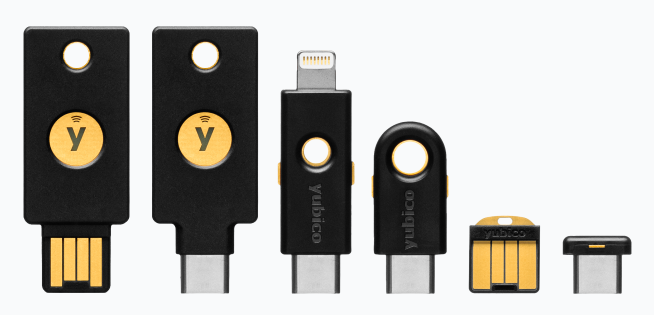
\includegraphics[width=0.95\textwidth]{assets/yubikey-5.png}
  \end{center}
  \caption[Verschiedene U2F Security Keys von Yubico.]{Verschiedene U2F Security Keys von Yubico (v.l.n.r.): YubiKey 5 NFC, YubiKey 5C NFC, YubiKey 5Ci, YubiKey 5 Nano und YubiKey 5C Nano.\\\parencite{yubicoYubiKeySeries2024}}
  \label{fig:yubikey}
\end{figure}

Die genannte Aktivierung wird von verschiedenen Herstellern unterschiedlich umgesetzt. Angeboten werden Produkte mit kapazitiven Touch-Sensoren (z.B. von Yubico, siehe Abbildung \ref{fig:yubikey}) oder mit mechanischen Knöpfen \parencite{langSecurityKeys2017}. Es existieren auch Geräte, die beim Einführen automatisch aktiviert werden, und somit für jede Authentifizierung erneut eingesteckt werden müssen \parencite{langSecurityKeys2017}.

Der \ac{U2F}-Standard wird über eine Public-Key-Private-Key-Architektur umgesetzt. Dabei wird vom Security Key bei der Registration ein öffentlicher Schlüssel erstellt, der an die Anwendung übermittelt wird \parencite{langSecurityKeys2017}. Der private Schlüssel verlässt das Gerät nie, und wird im tagtäglichen Gebrauch dazu genutzt, Zeichenketten zu erstellen, die mithilfe des öffentlichen Schlüssels überprüft werden können \parencite{reeseUsabilityStudy2019}.

\subsubsection{Sicherheitsaspekte}

Security Keys sind gegenüber den anderen \ac{2FA}-Methoden deutlich sicherer. Eine Durchführung von (Echtzeit-)Phishing-Attacken ist bei der Nutzung von \ac{U2F} nicht möglich \parencite{langSecurityKeys2017}. Shoulder-Surfing und Keylogging wird durch die Länge der Zeichenkette und ein Verzicht auf eine manuelle Eingabe erschwert. Des Weiteren werden viele Angriffsvektoren durch einen komplexen Transaktionsaufbau erschwert. Das \ac{U2F}-Protokoll arbeitet beispielsweise auch mit \textit{TLS Channel IDs}, welche genutzt werden können um die Echtheit der Antwort des Security Keys zu überprüfen \parencite{langSecurityKeys2017}. Somit werden sogar \ac{MIM}-Attacken erschwert \parencite{langSecurityKeys2017}.

Das Hauptrisiko bei der Nutzung von \ac{U2F} stellt ein Verlust oder Diebstahl des Security Keys dar, dies ist jedoch auch bei den zuvor genannten \ac{2FA}-Methode der Fall \parencite{reeseUsabilityStudy2019}. Ein gezielter Diebstahl ist jedoch zeit- und kostenintensiv und für die gleichzeitige Kompromittierung von vielen Accounts nicht praktikabel.

\subsubsection{Usability}

\ac{U2F} Security Keys weisen im Vergleich auf zu anderen \ac{2FA}-Methoden weniger Fehlerfälle auf \parencite{langSecurityKeys2017}, da eine manuelle Eingabe von Codes nicht benötigt wird. Auch der Nutzungsaufwand wird als gering angesehen, da nur ein Knopf gedrückt und der Security Key eingesteckt werden muss \parencite{langSecurityKeys2017}. Des Weiteren beschreibt \textcite{langSecurityKeys2017} die Funktionsweise von Security Keys als effizient und einfach zu erlernen.

Laut der Studie von \textcite{reeseUsabilityStudy2019} wurde die Verfügbarkeit des Security Keys als zusätzliche Hürde für die \ac{2FA} identifiziert. Je nach Aufbewahrungsmethode entstand so ein Mehraufwand, um das Gerät zu besorgen.

Schlussendlich werden \ac{U2F} Security Keys von \textcite{langSecurityKeys2017} als barrierearm beschrieben, da nur ein Knopfdruck erforderlich ist. Sehbehinderte Menschen müssen somit keine Zahlen ablesen und eintippen.
